\documentclass{article}

\title{Convolutional Neural Networks}
\author{John Chidiac}

\usepackage{listings}
\usepackage[margin=1.75in]{geometry}
\usepackage{diagbox}
\usepackage{amsmath}
\usepackage{graphicx}
\usepackage{algpseudocode}
\usepackage{tikz}
\usepackage{pgfplots}
\pgfplotsset{compat=1.18}
\usetikzlibrary{fillbetween, intersections}
\usetikzlibrary{arrows.meta, positioning, decorations.pathreplacing}
\usepackage{algorithm,algorithmicx,algpseudocode}
\usepackage{amssymb}
\usepackage[framemethod=TikZ]{mdframed}
\usepackage[linguistics]{forest}

\tikzset{arrowed/.style={decorate,
		decoration={show path construction, 
			moveto code={},
			lineto code={
				\draw[#1] (\tikzinputsegmentfirst) --  (\tikzinputsegmentlast);
			},
			curveto code={},
			closepath code={},
}},arrowed/.default={-stealth}}

\pgfplotsset{gradient function/.initial=f,
dx/.initial=0.01,dy/.initial=0.01}
\pgfmathdeclarefunction{xgrad}{2}{%
	\begingroup%
	\pgfkeys{/pgf/fpu,/pgf/fpu/output format=fixed}%
	\edef\myfun{\pgfkeysvalueof{/pgfplots/gradient function}}%
	\pgfmathparse{(\myfun(#1+\pgfkeysvalueof{/pgfplots/dx},#2)%
	-\myfun(#1,#2))/\pgfkeysvalueof{/pgfplots/dx}}%
	\pgfmathsmuggle\pgfmathresult\endgroup%
}

\pgfmathdeclarefunction{ygrad}{2}{%
	\begingroup%
	\pgfkeys{/pgf/fpu,/pgf/fpu/output format=fixed}%
	\edef\myfun{\pgfkeysvalueof{/pgfplots/gradient function}}%
	\pgfmathparse{(\myfun(#1,#2+\pgfkeysvalueof{/pgfplots/dy})%
	-\myfun(#1,#2))/\pgfkeysvalueof{/pgfplots/dy}}%
	\pgfmathsmuggle\pgfmathresult\endgroup%
}
\begin{document}
\maketitle
\thispagestyle{empty}
\pagebreak

\tableofcontents
\thispagestyle{empty}
\pagebreak

\pagenumbering{arabic}
\section{Basic Concepts in Machine Learning}
\subsection{Neurons}
A neuron is a mathematical function inspired by biological neurons. It receives one or more inputs and sums them to 
produce an output. Each input is separately weighted and the sum is passed through an activation function. They are often monotonically increasing, 
bounded, continuous, and differentiable.
\subsubsection{Basic Structure}
Given an artificial neuron $k$, we consider $m+1$ inputs with signals $x_0\to x_m$ and weights $w_{k0}\to w_{km}$. Typically 
we assign "$+1$" to $x_0$ which makes it a bias input with $w_{k0}=b_k$. This leaves $m$ actual inputs to the neuron. 
$\phi(\cdot)$ is the activation function, $v_k$ is our neuron, and $y_k$ is the output.

\vspace{-0.5cm}
\begin{figure}[h]
	\centering
	\begin{tikzpicture}[every node/.style={circle, draw, minimum size=0.01cm}, text node/.style={rectangle, draw=none}]

		\node[circle,draw] (input1) at (0, 1.5) {};
		\node[circle,draw] (input2) at (0, 0.5) {};
		\node[circle,draw] (input3) at (0, -0.5) {};
		\node[circle,draw] (input4) at (0, -2cm) {};

		\node[circle,draw] (hidden) at (3,0) {};

		\node[circle,draw] (output) at (6,0) {};

		\foreach \i in {1,2,3,4} {
			\draw[-] (input\i) -- (hidden);
		}

		\draw[-] (hidden) -- (output);

		\node[label=above:{$x_m$}, draw=none, yshift=-1.25cm] at (input4.north) {};
		\node[label=above:{$\vdots$}, draw=none, yshift=0cm] at (input4.north) {};
		\node[label=above:{$x_0$}, draw=none, yshift=-.25cm] at (input1.north) {};
		\node[label=above:{$x_1$}, draw=none, yshift=-.25cm] at (input2.north) {};
		\node[label=above:{$x_2$}, draw=none, yshift=-.25cm] at (input3.north) {};
		\node[label=above:{$v_k$}, draw=none, yshift=-0.25cm] at (hidden.north) {};
		\node[label=above:{$\phi(\cdot)$}, draw=none, yshift=-0.5cm, xshift = 1.5cm] at (hidden.north) {};
		\node[label=above:{$y_k$}, yshift=-0.25cm, draw=none] at (output.north) {};
	\end{tikzpicture}
\end{figure}
\vspace{-1cm}
\subsubsection{Implementing a Threshold Logic Unit}
A TLU is a type of artificial neuron that takes a set of binary inputs, applies a weight to them, sums them, subtracts 
a threshold value, then passes them through a step function. The TLU we look at is a very simple and elementary example.

\begin{algorithm}
	\floatname{algorithm}{Neuron}
	\caption{Threshold Logic Unit}\label{alg:TLU}
	\begin{algorithmic}[1]
		\State threshold $\gets$ number
		\State weights $\gets$ numbers[X]
		\Procedure{fire}{booleans[X]}
		\State T $\gets$ 0
		\For{i $\gets$ 1 to X}
		\If{booleans[i] = true}
		\State T $\gets$ T + weights[i]
		\EndIf
		\EndFor
		\State \Return T $>$ threshold
		\EndProcedure
	\end{algorithmic}
\end{algorithm}

\pagebreak

\subsection{Activation Functions}
The activation function of a node in a neural network is a function that calculates the output of the node based on 
its inputs and the weights on individual inputs. Nonlinear activation functions are essential to solve more complicated 
problems.
\subsubsection{Different Properties of Activation Functions}
\paragraph{Nonlinearity.} When the activation function is non-linear, then a two-layer neural network can be proven to 
be a universal function approximator by the \textit{Universal Approximation Theorem}. The identity function, which is 
linear, does not satisfy this property. When multiple layers use the identity function, the entire model is equivalent 
to a single-layer model.
\paragraph{Range.} When the range of the activation function is finite, gradient-based training methods tend to be more
stable, because pattern presentations significantly affect only limited weights. When the range is infinite, training is
generally more efficient because pattern presentations significantly affect most of the weights. In the case of infinite 
ranges, smaller learning rates are necessary.
\paragraph{Continuously Differentiable.} This property is desirable for enabling gradient-based optimization methods.

\subsubsection{Mathematical Details and Activation Functions}
A function $f$ is \textit{saturating} if $\lim_{|v|\to \infty}|\nabla f(v)| = 0$. Networks with non-saturating activation
functions may be better than saturating ones because they are less likely to suffer from the vanishing gradient problem. 
We have ridge activation functions:
\begin{itemize}
	\item Linear activation: $\phi(v)=a+v'b$
	\item ReLU activation: $\max(0, \phi(v)=a+v'b)$
	\item Heaviside activation: $\phi(v)=1$ if $a+v'b>0$
	\item Logistic activation: $\phi(v)=(1+\exp(-a-v'b))^{-1}$
\end{itemize}

\noindent Radial activation functions used in radial basis function networks:
\begin{itemize}
	\item Gaussian activation: $\phi(v)=\exp\left(-\frac{||v-c||^2}{2\sigma^2}\right)$
	\item Multiquadratic activation: $\phi(v)=\sqrt{||v-c||^2+a^2}$
	\item Inverse multiquadratic activation: $\phi(v)=\left(||v-c||^2+a^2\right)^{-\frac{1}{2}}$
\end{itemize}
\noindent And finally, folding activation functions.

\pagebreak

\subsection{Gradient Descent}
Gradient descent is a first-order iterative optimization algorithm for finding a local minimum of a differentiable function. 
The idea is to take repeated steps in the opposite direction of the gradient of the function at the current point. Doing 
otherwise will lead us to the local maximum. It is useful for minimizing the cost or loss function. 
\begin{figure}[H]
	\centering
	\begin{tikzpicture}
		\begin{axis}[width=10cm,height=7cm,
			declare function={f(\x,\y)=cos(deg(\x)*0.8)*cos(deg(\y)*0.6)*exp(0.1*\x);}]
			\addplot3[surf,shader=interp,domain=-4:3,%samples=81
			colormap/blackwhite, view={60}{45}]{f(x,y)};
			\edef\myx{1} % first x coordinate
			\edef\myy{0.25} % first y coordinate
			\edef\mystep{-0.25}% negative values mean descending
			\pgfmathsetmacro{\myf}{f(\myx,\myy)}
			\edef\lstCoords{(\myx,\myy,\myf)}
			\pgfplotsforeachungrouped\X in{0,...,5}
			{
				\pgfmathsetmacro{\mydx}{xgrad(\myx,\myy)}
				\pgfmathsetmacro{\mydy}{ygrad(\myx,\myy)}
				\pgfmathsetmacro{\myscale}{\mystep/sqrt(\mydx*\mydx+\mydy*\mydy)}
				\pgfmathsetmacro{\myx}{\myx+\myscale*\mydx}
				\pgfmathsetmacro{\myy}{\myy+\myscale*\mydy} 
				\pgfmathsetmacro{\myf}{f(\myx,\myy)}
				\edef\lstCoords{\lstCoords\space (\myx,\myy,\myf)}
			}
			\addplot3[samples y=0,arrowed] coordinates \lstCoords;
		\end{axis}
	\end{tikzpicture}
\end{figure}
\noindent Gradient descent is based on the observation that if a multivariable function $F(x)$ is defined and differentiable in a neighborhood 
of point $a$, then $F(x)$ decreases the fastest if one goes from $a$ in the direction of the negative gradient of $F$ at $a$,
$-\nabla F(a)$. Then, if $a_{n+1}=a_n-\gamma \nabla F(a_n)$ where $\gamma$ is the learning rate, for a small enough learning 
rate, $\gamma\in\mathbb{R}_+$, we have $F(a_n)\geq F(a_{n+1})$. With that observation, we have

\begin{equation}
	F(x_0)\geq F(x_1) \geq \dots \geq F(x_n)
	\label{eq:monotonicgradient}
\end{equation}

\noindent and we hope that the sequence $x_n$ converges to the desired local minimum.

\subsection{Learning Rate}
The learning rate is a tuning parameter in an optimization algorithm that determines the step size at each iteration 
while moving toward a minimum of a loss function. When setting a learning rate, there is a trade-off between the rate of 
convergence and overshooting. While the descent direction is determined by the gradient of the loss function, the learning 
rate determines how big a step is taken in that direction. Too high might jump above the minimum and too low may never reach 
it. In order to achieve faster convergence, prevent oscillations and getting stuck in undesirable local minima the 
learning rate is often varied during training either in accordance to a learning rate schedule or by using an adaptive 
learning rate.

\subsection{Loss Function}
A loss function is a function that maps an event or values of one or more variables onto a real number representing some 
cost associated with the event. Optimization algorithms seek to minimize the loss function. 
\subsubsection{Quadratic Loss Function}
The use of a quadratic loss function is common since it is often more mathematically manageable than other loss functions 
because of its symmetry and properties of variances. If the target is $t$, $x$ is the value predicted by the model, and $C$ is 
some constant scaling factor, then the squared error loss is:
\begin{equation}
	\lambda(x)=C(t-x)^2
	\label{eq:SEL}
\end{equation}

\subsubsection{0-1 Loss Function}
This loss function is most commonly used in statistics and uses the Iverson bracket notation (1 when true, 0 when false).
\begin{equation}
	L(\hat y, y)=[y\neq \hat y]
	\label{eq:01loss}
\end{equation}


\pagebreak
\section{Building a Neural Network}
The essential steps of machine learning are:
\begin{enumerate}
	\item Feed input $y=\text{network}(x,w)$
	\item Calculate the error $E = \frac{1}{2}(\hat y-y)^2$
	\item Adjust the parameters using gradient descent $w \gets w - \gamma\frac{\partial E}{\partial w}$
	\item Repeat
\end{enumerate}
\noindent where $W$ is a set of parameters that are updated with gradient descent.

\subsection{Implementation Design}
We want modular code, so we need to implement every layer separately. We need a model that fits every type of layer. A layer 
is just a large function. For every input we give a layer, we get an output. This is called \textit{forward propagation}. 
The next step is called \textit{backward propagation}. During backward propagation, if the layer is given the derivative of 
its error with respect to its output, $\frac{\partial E}{\partial Y}$, it gives back the derivative of the error with respect to 
its input $\frac{\partial E}{\partial X}$.
\begin{equation}
	\displaystyle\frac{\partial E}{\partial W} = \displaystyle\frac{\partial E}{\partial Y}\displaystyle\frac{\partial Y}{\partial W}
	\label{eq:derivativeoferrorwrtparameter}
\end{equation}
\noindent where
\begin{equation}
	\displaystyle\frac{\partial E}{\partial X} = \displaystyle\frac{\partial E}{\partial Y}\displaystyle\frac{\partial Y}{\partial X}
	\label{eq:derivativeoferrorwrtinput}
\end{equation}

\begin{figure}[h]
	\centering
	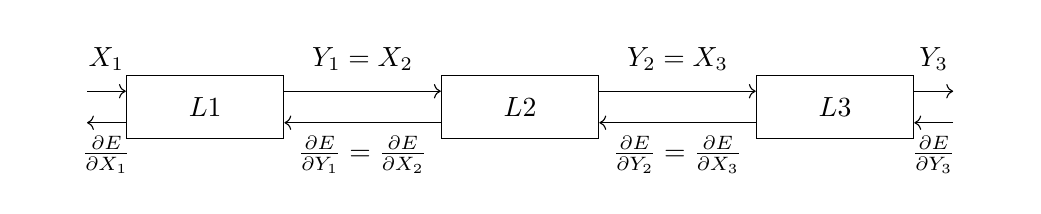
\begin{tikzpicture}[every node/.style={rectangle, draw, minimum width=2cm, minimum height = 0.8cm}, text node/.style={rectangle, draw=none}]
		\node (input1) at (0,0) {$L1$};
		\node (input2) at (4,0) {$L2$};
		\node (input3) at (8,0) {$L3$};
		\draw [->] ([yshift=0.2cm]input1.east) -- node[above, draw = none] {$Y_1 = X_2$} ([yshift=0.2cm]input2.west);
		\draw [->] ([yshift=0.2cm]input2.east) -- node[above, draw = none] {$Y_2 = X_3$} ([yshift=0.2cm]input3.west);
		\draw [->] (-1.5, 0.2cm) -- node[above, draw = none] {$X_1$} ([yshift=0.2cm]input1.west);
		\draw [->] ([yshift=0.2cm]input3.east) -- node[above, draw=none] {$Y_3$} (9.5, 0.2cm);
		\draw [->] ([yshift=-0.2cm]input2.west) -- node[below, draw = none] {$\frac{\partial E}{\partial Y_1} = \frac{\partial E}{\partial X_2}$} ([yshift=-0.2cm]input1.east);
		\draw [->] ([yshift=-0.2cm]input3.west) -- node[below, draw = none] {$\frac{\partial E}{\partial Y_2} = \frac{\partial E}{\partial X_3}$} ([yshift=-0.2cm]input2.east);
		\draw [->] (9.5, -0.2cm) -- node[below, draw = none] {$\frac{\partial E}{\partial Y_3}$} ([yshift=-0.2cm]input3.east);
		\draw [->] ([yshift=-0.2cm]input1.west) -- node[below, draw = none] {$\frac{\partial E}{\partial X_1}$} (-1.5, -0.2cm);
	\end{tikzpicture}
\end{figure}

\subsection{The Dense Layer}

In the dense layer, every input neuron is connected to every output neuron. Each connection represents a weight $w_{ji}$, or 
the weight that connects the output neuron $j$ to the output neuron $i$. The bias $b_j$ is a trainable parameter. The below is 
the \textit{forward propagation}.
\begin{equation}
	y_j=\displaystyle\sum_{k=1}^{i}x_k w_{jk} + b_j
	\label{eq:outputsum}
\end{equation}

\pagebreak

\noindent We can write $y_1 \to y_j$ using matrices for simplicity and ease of computation:

\begin{equation}
	\begin{bmatrix} 
		y_1 \\ y_2 \\ \vdots \\ y_j
	\end{bmatrix} =
	\begin{bmatrix}
		w_{11} & w_{12} & \dots & w_{1i} \\
		w_{21} & w_{22} & \dots & w{2i} \\
		\vdots & \vdots & \ddots &\vdots \\
		w_{j1} & w_{j2} & \dots & w_{ji}
	\end{bmatrix}
	\begin{bmatrix} 
		x_1 \\ x_2 \\ \vdots \\ x_j
	\end{bmatrix} + 
	\begin{bmatrix} 
		b_1 \\ b_2 \\ \vdots \\ b_j
	\end{bmatrix} 
	\label{eq:outputsummatrix}
\end{equation}

\noindent Now, we look at the backward step, \textit{back propagation}. Given the error of the output of the depth layer, 
we need the derivative of the error with respect to the weights and biases, since these are the trainable parameters. Next, 
we need the error with respect to the input since it will be passed to the layer before the one computing the dense layer.

\begin{align}
	\displaystyle\frac{\partial E}{\partial Y}&=\begin{bmatrix}
		\frac{\partial E}{\partial y_1} 
		\vspace{0.2cm} \\
		\frac{\partial E}{\partial y_2} \\
		\vdots \\
		\frac{\partial E}{\partial y_j}
	\end{bmatrix} &
		\displaystyle\frac{\partial E}{\partial W}&=\begin{bmatrix}
			\frac{\partial E}{\partial w_{11}} &
			\frac{\partial E}{\partial w_{12}} &
			\dots &
			\frac{\partial E}{\partial w_{1i}}
			\vspace{0.2cm} \\
			\frac{\partial E}{\partial w_{21}} &
			\frac{\partial E}{\partial w_{22}} &
			\dots &
			\frac{\partial E}{\partial w_{2i}} \\
			\vdots & \vdots & \ddots & \vdots \\
			\frac{\partial E}{\partial w_{j1}} &
			\frac{\partial E}{\partial w_{j2}} &
			\dots &
			\frac{\partial E}{\partial w_{ji}} \\
		\end{bmatrix}
	\label{eq:errors}
\end{align}

\noindent but, $\frac{\partial E}{\partial w_{ji}} = \frac{\partial E}{\partial y_j}x_i$

\begin{equation}
	\displaystyle\frac{\partial E}{\partial W} = 
	\begin{bmatrix}
		\frac{\partial E}{\partial y_1} 
		\vspace{0.2cm} \\
		\frac{\partial E}{\partial y_2} \\
		\vdots \\
		\frac{\partial E}{\partial y_j}
	\end{bmatrix}
	\begin{bmatrix}
		x_1 & x_2 & \dots & x_n 
	\end{bmatrix} = \displaystyle\frac{\partial E}{\partial Y}X^t
	\label{eq:errorwrtweightsandbiases}
\end{equation}

\noindent where $X^t$ is $X$ transposed. Moreover,

\begin{equation}
	\frac{\partial E}{\partial b_j} = \frac{\partial E}{\partial y_j} \iff 
	\frac{\partial E}{\partial B} = \frac{\partial E}{\partial Y}
	\label{eq:errorwrtbias}
\end{equation}

\noindent And finally,

\begin{equation}
	\frac{\partial E}{\partial X}=\begin{bmatrix}
		w_{11} & w_{21} & \dots & w_{j1} \\
		w_{12} & w_{22} & \dots & w_{j2} \\
		\vdots & \vdots & \ddots & \vdots \\
		w_{1i} & w_{2i} & \dots & w_{ji}
	\end{bmatrix}
	\begin{bmatrix}
		\frac{\partial E}{\partial y_1} 
		\vspace{0.2cm} \\
		\frac{\partial E}{\partial y_2} \\
		\vdots \\
		\frac{\partial E}{\partial y_j}
	\end{bmatrix} = W^t\displaystyle\frac{\partial E}{\partial Y}
	\label{eq:errorwrtoutput}
\end{equation}

\pagebreak

\subsection{The Activation Layer}

\begin{figure}[h]
	\centering
	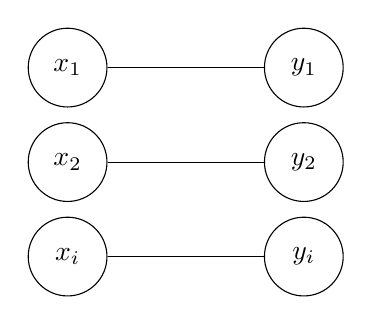
\begin{tikzpicture}[every node/.style={circle, draw, minimum width=1cm}, text node/.style={rectangle, draw=none}]
		\node (x1) at (0,2.4) {$x_1$};
		\node (y1) at (3,2.4) {$y_1$};
		\node (x2) at (0,1.2) {$x_2$};
		\node (y2) at (3,1.2) {$y_2$};
		\node (x3) at (0,0) {$x_i$};
		\node (y3) at (3,0) {$y_i$};

		\draw [-] (x1) -- (y1) {};
		\draw [-] (x2) -- (y2) {};
		\draw [-] (x3) -- (y3) {};
	\end{tikzpicture}
\end{figure}

\noindent The \textit{forward propagation} of the activation layer is described by
\begin{equation}
	Y=f(X)
	\label{eq:forwardactivation}
\end{equation}

\noindent From equation (\ref{eq:forwardactivation}), we have
\begin{equation}
	\displaystyle\frac{\partial E}{\partial X} =
	\displaystyle\frac{\partial E}{\partial Y} \odot f'(X)
	\label{eq:errorwrtoutputactivation}
\end{equation}

\pagebreak

\section{Building a Convolutional Neural Network}

\subsection{Cross-Corrolation and Convolution}

The equation described below is known as valid cross-corrolation.

\begin{equation}
	\underset{\text{input}}{
		\begin{bmatrix}
			1 & 6 & 2 \\
			5 & 3 & 1 \\
			7 & 0 & 4
	\end{bmatrix}} \star
	\underset{\text{kernel}}{
		\begin{bmatrix}
			1 & 2 \\
			-1 & 0
		\end{bmatrix}
	} = \underset{\text{output}}{
		\begin{bmatrix}
			8 & 7 \\
			4 & 5
	\end{bmatrix}}
	\label{eq:validcrosscorrolation}
\end{equation}

\noindent We note that the $\star$ operator denotes cross-corrolation. From the above, by rotating the kernel 
by 180 degrees, we can get the convolution:

\begin{equation}
	\text{conv}(I, K) = I \star rot180(K)
	\label{eq:convolution}
\end{equation}

\noindent Now, we introduce full cross-corrolation. This starts whenever the kernel intersects with the input, 
in the case before, it only worked with full intersection.

\begin{equation}
	\underset{\text{input}}{
		\begin{bmatrix}
			1 & 6 & 2 \\
			5 & 3 & 1 \\
			7 & 0 & 4
	\end{bmatrix}} \underset{\text{full}}{\star}
	\underset{\text{kernel}}{
		\begin{bmatrix}
			1 & 2 \\
			-1 & 0
		\end{bmatrix}
	} = \underset{\text{output}}{
		\begin{bmatrix}
			0 & -1 & -6 & -2 \\
			2 & 8 & 7 & 1 \\
			10 & 4 & 5 & -3 \\
			14 & 7 & 8 & 4
		\end{bmatrix}
	}
	\label{eq:fullcrosscorrolation}
\end{equation}

\subsection{The Convolutional Layer}

The convolutional layer takes in a 3 dimensional array as input which may have depth. The layer has trainable parameters 
such as the kernels and biases. This produces an output with the same depth as the kernel. Below, we describe the 
\textit{forward propagation} of a convolutional neural network.

\begin{equation}
	Y_i = B_i + \displaystyle\sum_{j=1}^{n}X_j\star K_{ij}
	\label{eq:forwardpropagationoftheconvolutionallayer}
\end{equation}

\noindent Now, we find the necessary derivatives for \textit{backward propagation}.

\begin{align}
	\displaystyle\frac{\partial E}{\partial K_{ij}} &= X_j \star \displaystyle\frac{\partial E}{\partial Y_i} \\
	\displaystyle\frac{\partial E}{\partial B_i} &= \displaystyle\frac{\partial E}{\partial Y_i} \\
	\displaystyle\frac{\partial E}{\partial X_j} &= \displaystyle\sum_{i=1}^{n}
	\displaystyle\frac{\partial E}{\partial Y_i} \underset{\text{full}}{*} K_{ij}
	\label{eq:kernelbackpropagation}
\end{align}

\pagebreak

\subsection{Cross-Entropy}

\subsubsection{Binary Cross-Entropy Loss}
Binary cross-entropy loss is a loss function for binary datasets defined as

\begin{equation}
	E=-\frac{1}{n}\displaystyle\sum_{i=1}^{n}\hat y_i\log(y_i)+(1-\hat y_i)\log(1-y_i)
	\label{eq:binarycrossentropyloss}
\end{equation}

\noindent Its derivative with respect to $y$ is described as

\begin{equation}
	\displaystyle\frac{\partial E}{\partial y_i}=\frac{1}{n}\left(\displaystyle\frac{1-\hat y_i}{1-y_i}-\displaystyle\frac{\hat y_i}{y_i}\right)
	\label{eq:binarycrossentropylossprime}
\end{equation}

\noindent For this type of problem, we typically use the sigmoid activation function.

\begin{align}
	\sigma(x) &= \frac{1}{1+e^{-x}} \\
	\sigma'(x) &= \sigma(x) \times (1-\sigma(x))
\end{align}

\end{document}
